%%%%%%%%%%%%%%%%%%%%%%%%%%%%%%%%%%%%%%%%%%%%%%%%%%%%%%%%%%%%%%%%%%%%%%%%%%%%%%%%%%
\begin{frame}[fragile]\frametitle{}
\begin{center}
{\Large Jottings from Talks, Tweets}

{\small Dr Shiva Ayyadurai}


\end{center}
\end{frame}

%%%%%%%%%%%%%%%%%%%%%%%%%%%%%%%%%%%%%%%%%%%%%%%%%%%%%%%%%%%%%%%%%%%%%%%%%%%%%%%%%%
\begin{frame}[fragile]\frametitle{}
\begin{center}
{\Large Dr.SHIVA: SHATTER THE SWARM. How The Few Control the Many.}
\end{center}
\end{frame}


%%%%%%%%%%%%%%%%%%%%%%%%%%%%%%%%%%%%%%%%%%%%%%%%%%%%%%%%%%%%%%%%%%%%%%%%%%%%%%%%%%
\begin{frame}[fragile]\frametitle{Introduction}
    \begin{itemize}
        \item Dr. Shiva discusses how a small group of elites control 8 billion people.
        \item The elite consists of roughly 10,000 individuals.
        \item Swarm intelligence helps elites manipulate large populations.
        \item Their primary goal is power, profit, and control.
    \end{itemize}
\end{frame}

%%%%%%%%%%%%%%%%%%%%%%%%%%%%%%%%%%%%%%%%%%%%%%%%%%%%%%%%%%%%%%%%%%%%%%%%%%%%%%%%%%
\begin{frame}[fragile]\frametitle{Elite Control Systems}
    \begin{itemize}
        \item Elites use control systems to manipulate the population.
        \item Inputs include: unhealthy, ignorant, entertained, isolated, and helpless people.
        \item Outputs sought: disorganization, helplessness, and dependency on elites.
    \end{itemize}
\end{frame}

%%%%%%%%%%%%%%%%%%%%%%%%%%%%%%%%%%%%%%%%%%%%%%%%%%%%%%%%%%%%%%%%%%%%%%%%%%%%%%%%%%
\begin{frame}[fragile]\frametitle{Interconnected Elites}
    \begin{itemize}
        \item Elites form a tightly knit, interconnected group.
        \item They share personal connections, frequent the same locations, and maintain close relationships.
        \item They influence academia, government, NGOs, and big corporations.
    \end{itemize}
\end{frame}

%%%%%%%%%%%%%%%%%%%%%%%%%%%%%%%%%%%%%%%%%%%%%%%%%%%%%%%%%%%%%%%%%%%%%%%%%%%%%%%%%%
\begin{frame}[fragile]\frametitle{Key Institutions of Power}
    \begin{itemize}
        \item Elites control major institutions: academia (Harvard, IIT), NGOs (Clinton Initiative), and government bodies (CIA, think tanks).
        \item CEOs of global companies like Pfizer and JPMorgan are part of the elite group.
        \item Hollywood, media, and social media influencers are also key components.
    \end{itemize}
\end{frame}

%%%%%%%%%%%%%%%%%%%%%%%%%%%%%%%%%%%%%%%%%%%%%%%%%%%%%%%%%%%%%%%%%%%%%%%%%%%%%%%%%%
\begin{frame}[fragile]\frametitle{Manipulating the Public}
    \begin{itemize}
        \item Elites manipulate policies and public perception through propaganda.
        \item False heroes like Trump, Kennedy, and Gandhi are created to serve elite interests.
        \item The goal is to ensure people remain divided and helpless, seeking elites as saviors.
    \end{itemize}
\end{frame}

%%%%%%%%%%%%%%%%%%%%%%%%%%%%%%%%%%%%%%%%%%%%%%%%%%%%%%%%%%%%%%%%%%%%%%%%%%%%%%%%%%
\begin{frame}[fragile]\frametitle{Dysfunction as a Goal}
    \begin{itemize}
        \item Elites foster dysfunction through societal issues like obesity, low testosterone, and confusion over identity.
        \item Life expectancy has decreased, reflecting the success of elite control over health and society.
        \item Policies and propaganda perpetuate these dysfunctions, ensuring continued profit for big pharma and other industries.
    \end{itemize}
\end{frame}

%%%%%%%%%%%%%%%%%%%%%%%%%%%%%%%%%%%%%%%%%%%%%%%%%%%%%%%%%%%%%%%%%%%%%%%%%%%%%%%%%%
\begin{frame}[fragile]\frametitle{Endocrine Disruption}
    \begin{itemize}
        \item Research shows chemicals like atrazine cause endocrine disruption, lowering testosterone levels.
        \item The investment community is complicit in supporting such industries, ensuring continued profit.
        \item Elites normalize dysfunction to prevent public awareness and preserve profits.
    \end{itemize}
\end{frame}

%%%%%%%%%%%%%%%%%%%%%%%%%%%%%%%%%%%%%%%%%%%%%%%%%%%%%%%%%%%%%%%%%%%%%%%%%%%%%%%%%%
\begin{frame}[fragile]\frametitle{Creating Division}
    \begin{itemize}
        \item Elites ensure division within society, using media and influencers to provoke different factions (pro-fat vs. anti-fat).
        \item They manipulate the narrative, ensuring that people remain distracted and divided.
        \item This division prevents collective action against the elites' control system.
    \end{itemize}
\end{frame}

%%%%%%%%%%%%%%%%%%%%%%%%%%%%%%%%%%%%%%%%%%%%%%%%%%%%%%%%%%%%%%%%%%%%%%%%%%%%%%%%%%
\begin{frame}[fragile]\frametitle{The Elite's Goal: Power, Profit, Control}
    \begin{itemize}
        \item The elites aim to maintain power through control over media, government, and key industries.
        \item They seek profit by fostering dependency, dysfunction, and division.
        \item The ultimate goal is to prevent people from organizing and seeking alternative leadership.
    \end{itemize}
\end{frame}

%%%%%%%%%%%%%%%%%%%%%%%%%%%%%%%%%%%%%%%%%%%%%%%%%%%%%%%%%%%%%%%%%%%%%%%%%%%%%%%%%%
\begin{frame}[fragile]\frametitle{Breaking Free: Understanding System Science}
    \begin{itemize}
        \item The way out is understanding the science of systems, which reveals how elites control society.
        \item Awareness of these principles is key to breaking free from elite manipulation.
        \item The principles of system science can be learned at Truth Freedom Health.
    \end{itemize}
\end{frame}

%%%%%%%%%%%%%%%%%%%%%%%%%%%%%%%%%%%%%%%%%%%%%%%%%%%%%%%%%%%%%%%%%%%%%%%%%%%%%%%%%%
\begin{frame}[fragile]\frametitle{Taking Action}
    \begin{itemize}
        \item To break free, become aware and get involved in initiatives that promote system science.
        \item Volunteer and support organizations like Truth Freedom Health.
        \item Knowledge and collective action are the tools to overcome elite control.
    \end{itemize}
\end{frame}

%%%%%%%%%%%%%%%%%%%%%%%%%%%%%%%%%%%%%%%%%%%%%%%%%%%%%%%%%%%
\begin{frame}[fragile]\frametitle{Summary pic}

\begin{center}
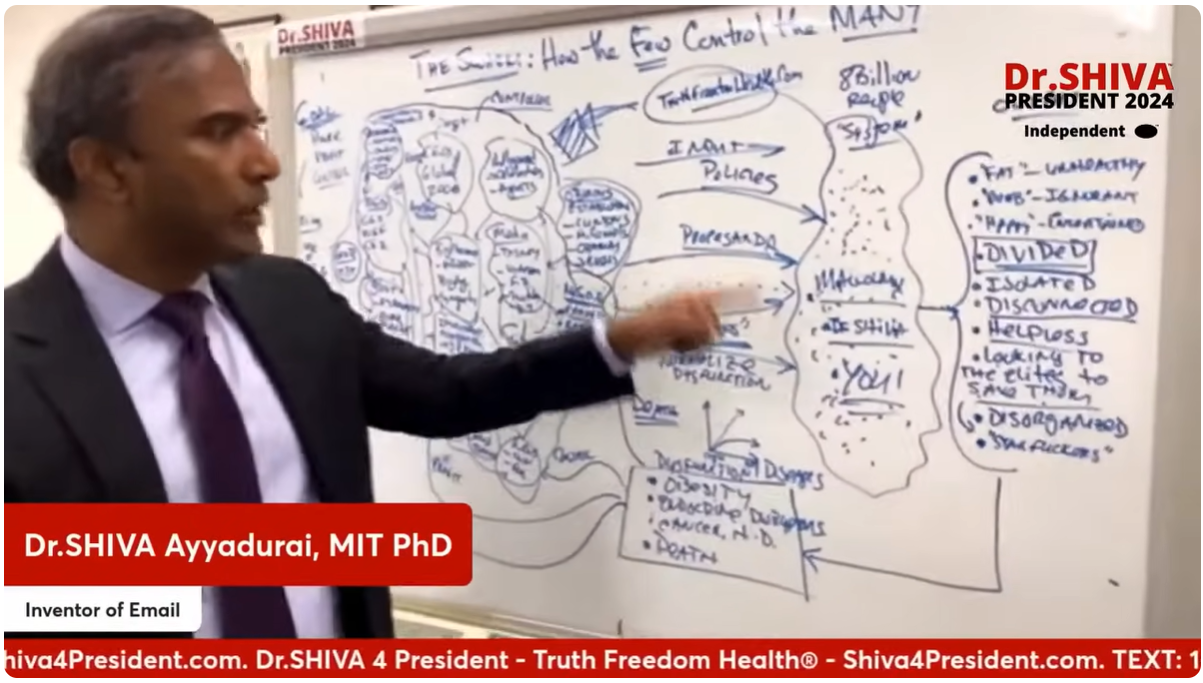
\includegraphics[width=\linewidth,keepaspectratio]{drshiva1}
\end{center}	  
\end{frame}

%%%%%%%%%%%%%%%%%%%%%%%%%%%%%%%%%%%%%%%%%%%%%%%%%%%%%%%%%%%%%%%%%%%%%%%%%%%%%%%%%%
\begin{frame}[fragile]\frametitle{}
\begin{center}
{\Large Dr.SHIVA: How The Swarm Is Killing You \& Your Children Even Sooner}
\end{center}
\end{frame}

%%%%%%%%%%%%%%%%%%%%%%%%%%%%%%%%%%%%%%%%%%%%%%%%%%%%%%%%%%%
\begin{frame}[fragile]\frametitle{Introduction to the Swarm}
      \begin{itemize}
          \item The "Swarm" is a decentralized, global system, not confined to any one individual, religion, or organization.
          \item It includes both the "obvious" and "not so obvious" establishments that control society.
          \item The "obvious establishment" includes known figures such as political leaders and royals.
          \item The "not so obvious establishment" includes figures like Robert Kennedy, Trump, AOC, and others who mask their true motives.
      \end{itemize}
\end{frame}

%%%%%%%%%%%%%%%%%%%%%%%%%%%%%%%%%%%%%%%%%%%%%%%%%%%%%%%%%%%
\begin{frame}[fragile]\frametitle{Effects of the Swarm’s Policies}
      \begin{itemize}
          \item The Swarm creates policies that harm the biological health of society.
          \item These policies have led to early death, obesity, immune system destruction, and reduced lifespans.
          \item Lifespan trends in the U.S. show a decline from 1980 to 2023.
          \item These policies disproportionately harm children, who are dying younger than previous generations.
      \end{itemize}
\end{frame}

%%%%%%%%%%%%%%%%%%%%%%%%%%%%%%%%%%%%%%%%%%%%%%%%%%%%%%%%%%%
\begin{frame}[fragile]\frametitle{The Not-So-Obvious Establishment}
      \begin{itemize}
          \item Figures like Kennedy, Trump, Bernie Sanders, and Al Sharpton are part of the "not so obvious establishment."
          \item These individuals disguise themselves as allies while supporting harmful policies.
          \item They benefit from the same systems that exploit working-class people.
      \end{itemize}
\end{frame}

%%%%%%%%%%%%%%%%%%%%%%%%%%%%%%%%%%%%%%%%%%%%%%%%%%%%%%%%%%%
\begin{frame}[fragile]\frametitle{Biological Triggers of Harm}
      \begin{itemize}
          \item Policies by the Swarm have led to biological dysfunctions such as mitochondrial damage, autophagy dysfunction, and oxidative stress.
          \item These dysfunctions contribute to early death and a weakened immune system.
          \item Molecular pathways affected include reduced NAD+ levels, autophagy gene downregulation, and increased oxidative stress markers.
      \end{itemize}
\end{frame}

%%%%%%%%%%%%%%%%%%%%%%%%%%%%%%%%%%%%%%%%%%%%%%%%%%%%%%%%%%%
\begin{frame}[fragile]\frametitle{Impact of Lockdowns}
      \begin{itemize}
          \item The Swarm’s policy of lockdowns led to stress, obesity, loneliness, depression, and poor nutrition.
          \item Both the obvious and not-so-obvious establishments supported these lockdowns.
          \item These lockdowns had devastating effects on people's physical and mental health.
      \end{itemize}
\end{frame}

%%%%%%%%%%%%%%%%%%%%%%%%%%%%%%%%%%%%%%%%%%%%%%%%%%%%%%%%%%%
\begin{frame}[fragile]\frametitle{The Monsanto Protection Act}
      \begin{itemize}
          \item The Monsanto Protection Act allowed the destruction of the environment and the creation of genetically engineered foods.
          \item This act led to poor nutrition and environmental pollution, worsening the health crisis.
          \item Key political figures, including Elizabeth Warren, supported this act, showing the unity of both political parties in harmful policies.
      \end{itemize}
\end{frame}

%%%%%%%%%%%%%%%%%%%%%%%%%%%%%%%%%%%%%%%%%%%%%%%%%%%%%%%%%%%
\begin{frame}[fragile]\frametitle{Healthcare and Economic Inequality}
      \begin{itemize}
          \item Group Purchasing Organizations (GPOs) and Pharmacy Benefit Managers (PBMs) expanded the healthcare system, increasing costs and reducing access.
          \item The result was more inequality, with wealth being transferred from working people to the elites.
          \item The pandemic worsened this inequality, with 600 billionaires increasing their wealth by \$2.3 trillion.
      \end{itemize}
\end{frame}

%%%%%%%%%%%%%%%%%%%%%%%%%%%%%%%%%%%%%%%%%%%%%%%%%%%%%%%%%%%
\begin{frame}[fragile]\frametitle{Environmental and Societal Damage}
      \begin{itemize}
          \item Factory farming, supported by the elites, contributed to poor nutrition and health problems.
          \item Imperialist wars caused stress, PTSD, and long-term societal harm.
          \item Environmental pollution, including noise and chemicals, exacerbated these issues.
      \end{itemize}
\end{frame}

%%%%%%%%%%%%%%%%%%%%%%%%%%%%%%%%%%%%%%%%%%%%%%%%%%%%%%%%%%%
\begin{frame}[fragile]\frametitle{The Biological Pathways Affected}
      \begin{itemize}
          \item Mitochondrial dysfunction leads to reduced NAD$+$ levels, affecting energy and immune function.
          \item Autophagy dysfunction impairs the body’s ability to repair cells.
          \item Oxidative stress increases reactive oxygen species, contributing to disease and early death.
          \item Inflammation, marked by CRP and COX-2, is another result of these policies.
      \end{itemize}
\end{frame}

%%%%%%%%%%%%%%%%%%%%%%%%%%%%%%%%%%%%%%%%%%%%%%%%%%%%%%%%%%%
\begin{frame}[fragile]\frametitle{Conclusion and Call to Action}
      \begin{itemize}
          \item The Swarm’s policies have systematically weakened our biology and society.
          \item These policies are a deliberate strategy by elites to maintain control and profit from dysfunction.
          \item To overcome this, people must awaken, reject the establishment, and get involved in the movement for truth, freedom, and health.
          \item Support the movement by engaging with educational resources and spreading awareness.
      \end{itemize}
\end{frame}


%%%%%%%%%%%%%%%%%%%%%%%%%%%%%%%%%%%%%%%%%%%%%%%%%%%%%%%%%%%
\begin{frame}[fragile]\frametitle{Summary pic}

\begin{center}
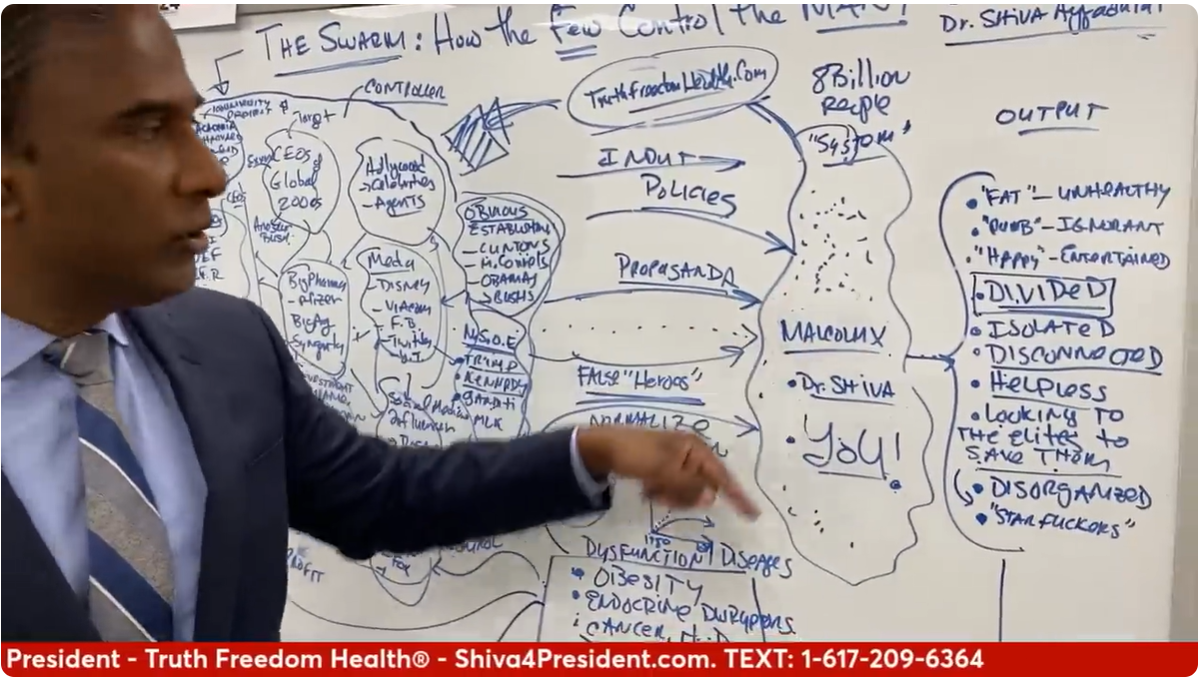
\includegraphics[width=\linewidth,keepaspectratio]{drshiva2}
\end{center}	  
\end{frame}


%%%%%%%%%%%%%%%%%%%%%%%%%%%%%%%%%%%%%%%%%%%%%%%%%%%%%%%%%%%%%%%%%%%%%%%%%%%%%%%%%%
\begin{frame}[fragile]\frametitle{}
\begin{center}
{\Large Dr.SHIVA: How THE Elites Enslave You Into One of Their 4 BUCKETS}
\end{center}
\end{frame}


%%%%%%%%%%%%%%%%%%%%%%%%%%%%%%%%%%%%%%%%%%%%%%%%%%%%%%%%%%%
\begin{frame}[fragile]\frametitle{Four Buckets of Control by the Establishment}
      \begin{itemize}
        \item The ruling class divides people into four buckets for control.
        \item \textbf{Bucket 1: Left Wing} 
        \begin{itemize}
            \item Includes parties like Labour (UK), Congress (India), and Democrats (USA).
            \item Promotes working-class division based on specific agendas.
        \end{itemize}
        \item \textbf{Bucket 2: Right Wing} 
        \begin{itemize}
            \item Includes parties like Tories (UK), BJP (India), and Republicans (USA).
            \item Creates opposition to left-wing policies, maintaining the divide.
        \end{itemize}
      \end{itemize}
\end{frame}

%%%%%%%%%%%%%%%%%%%%%%%%%%%%%%%%%%%%%%%%%%%%%%%%%%%%%%%%%%%
\begin{frame}[fragile]\frametitle{Other Buckets: Isolation and Terrorism}
      \begin{itemize}
        \item \textbf{Bucket 3: Apathetic and Isolationist}
        \begin{itemize}
            \item People disengage, focusing only on personal and family matters.
            \item Results in passive acceptance of the status quo.
        \end{itemize}
        \item \textbf{Bucket 4: Domestic Terrorists}
        \begin{itemize}
            \item People resort to violence out of desperation.
            \item Used as justification for increased control, like restricting free speech.
        \end{itemize}
      \end{itemize}
\end{frame}

%%%%%%%%%%%%%%%%%%%%%%%%%%%%%%%%%%%%%%%%%%%%%%%%%%%%%%%%%%%
\begin{frame}[fragile]\frametitle{Impact of the Four Buckets}
      \begin{itemize}
        \item Left and Right Wings split the working class into opposing factions.
        \item Apathetic individuals provide no challenge to the establishment.
        \item Domestic terrorism offers the ruling class excuses to suppress freedoms.
        \item These buckets ensure continued control by the establishment.
      \end{itemize}
\end{frame}

%%%%%%%%%%%%%%%%%%%%%%%%%%%%%%%%%%%%%%%%%%%%%%%%%%%%%%%%%%%
\begin{frame}[fragile]\frametitle{The Way Out: Building a Movement}
      \begin{itemize}
        \item \textbf{Truth, Freedom, and Health Movement} as the solution.
        \item Educating working-class people on the \textbf{science of systems}.
        \item Encourages understanding beyond left and right ideologies.
        \item Aims for conscious, community-driven innovation.
      \end{itemize}
\end{frame}

%%%%%%%%%%%%%%%%%%%%%%%%%%%%%%%%%%%%%%%%%%%%%%%%%%%%%%%%%%%
\begin{frame}[fragile]\frametitle{Historical Insights: Lessons from the Past}
      \begin{itemize}
        \item Early 1900s: Hygiene, clean water, and infrastructure reduced mortality.
        \item Achievements like labor rights emerged from Bottom-Up movements.
        \item Women-led labor movements unified people beyond ideological divides.
        \item A systems approach led to sustained societal improvements.
      \end{itemize}
\end{frame}

%%%%%%%%%%%%%%%%%%%%%%%%%%%%%%%%%%%%%%%%%%%%%%%%%%%%%%%%%%%
\begin{frame}[fragile]\frametitle{Unified Consciousness for Real Change}
      \begin{itemize}
        \item Raising individual and collective consciousness is essential.
        \item Encourages addressing root causes of problems through systemic thinking.
        \item Building community accelerates innovation and actionable solutions.
        \item A unified working class challenges the establishment's divide-and-rule.
      \end{itemize}
\end{frame}


%%%%%%%%%%%%%%%%%%%%%%%%%%%%%%%%%%%%%%%%%%%%%%%%%%%%%%%%%%%
\begin{frame}[fragile]\frametitle{Summary pic}

\begin{center}
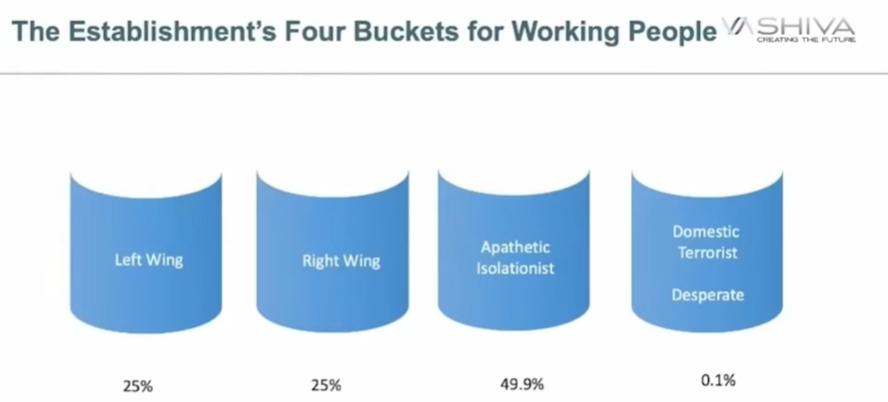
\includegraphics[width=\linewidth,keepaspectratio]{drshiva3}
\end{center}	  
\end{frame}

%%%%%%%%%%%%%%%%%%%%%%%%%%%%%%%%%%%%%%%%%%%%%%%%%%%%%%%%%%%%%%%%%%%%%%%%%%%%%%%%%%
\begin{frame}[fragile]\frametitle{}
\begin{center}
{\Large The Rosetta Stone of Ayurveda systems health}

{\small Dr Shiva Ayyadurai}


\end{center}
\end{frame}

%%%%%%%%%%%%%%%%%%%%%%%%%%%%%%%%%%%%%%%%%%%%%%%%%%%%%%%%%%%
\begin{frame}[fragile]\frametitle{Introduction to Systems Thinking}
      \begin{itemize}
        \item Explore connections between engineering systems and ancient Indian medicine (Ayurveda and Siddha).
        \item Ayurveda (Northern India) and Siddha (Southern India) practiced for 5000 years.
        \item Recent study validates the scientific foundation of these systems.
        \item Focus on holistic understanding of the body, contrasting with Western reductionist approaches.
        \item Control Systems Engineering bridges ancient and modern perspectives.
      \end{itemize}
\end{frame}

%%%%%%%%%%%%%%%%%%%%%%%%%%%%%%%%%%%%%%%%%%%%%%%%%%%%%%%%%%%
\begin{frame}[fragile]\frametitle{Core Concepts in Ayurveda and Siddha}
      \begin{itemize}
        \item Holistic approach rooted in personalized medicine.
        \item Key terms: 
          \begin{itemize}
            \item \textbf{Unmanifest energy (Prusha)} gives rise to gross elements (Prakriti).
            \item \textbf{Gunas}: Sattva (balance), Rajas (activity), Tamas (inertia).
            \item \textbf{Pancha Bhootas}: Earth, Water, Fire, Air, Ether.
            \item \textbf{Tridoshas}: Vata (motion), Pitta (transformation), Kapha (structure).
          \end{itemize}
        \item Western science struggles to align with these ancient terminologies.
      \end{itemize}
\end{frame}


%%%%%%%%%%%%%%%%%%%%%%%%%%%%%%%%%%%%%%%%%%%%%%%%%%%%%%%%%%%
\begin{frame}[fragile]\frametitle{Ayurveda Summary}

\begin{center}
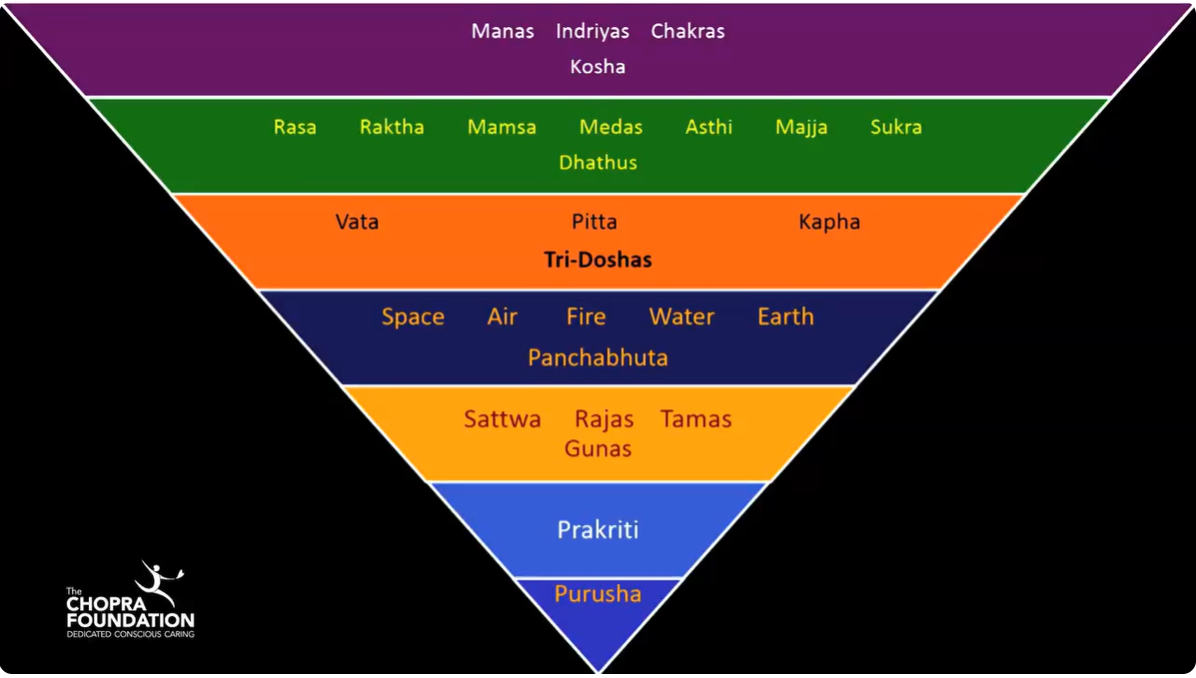
\includegraphics[width=\linewidth,keepaspectratio]{AyurvedaSummary}
\end{center}	  
\end{frame}

%%%%%%%%%%%%%%%%%%%%%%%%%%%%%%%%%%%%%%%%%%%%%%%%%%%%%%%%%%%
\begin{frame}[fragile]\frametitle{Control Systems Engineering Overview}
      \begin{itemize}
        \item Universal principles of all systems: 
          \begin{itemize}
            \item \textbf{Transport}: Movement or flow.
            \item \textbf{Conversion}: Transformation processes.
            \item \textbf{Storage}: Preservation or containment.
          \end{itemize}
        \item Examples: iPhones, thermostats, aircraft, human physiology.
        \item Intelligent systems involve goals, sensors, controllers, and feedback loops.
      \end{itemize}
\end{frame}

%%%%%%%%%%%%%%%%%%%%%%%%%%%%%%%%%%%%%%%%%%%%%%%%%%%%%%%%%%%
\begin{frame}[fragile]\frametitle{Systems Diagram}

\begin{center}
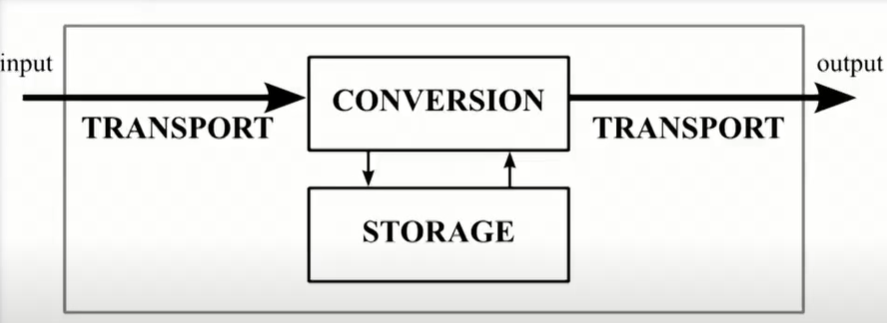
\includegraphics[width=0.8\linewidth,keepaspectratio]{SystemsDiagram}

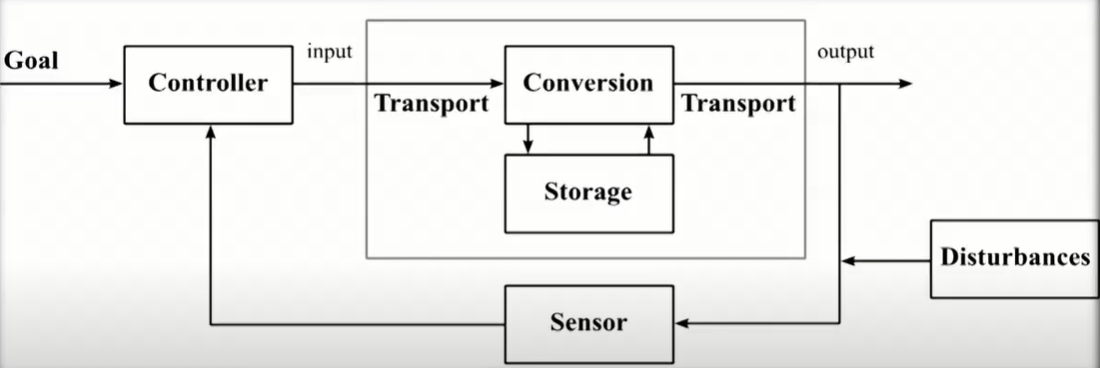
\includegraphics[width=0.8\linewidth,keepaspectratio]{SystemsDiagram_Intelligent}

\end{center}	  
\end{frame}

%%%%%%%%%%%%%%%%%%%%%%%%%%%%%%%%%%%%%%%%%%%%%%%%%%%%%%%%%%%
\begin{frame}[fragile]\frametitle{Systems Diagram Example}

\begin{center}
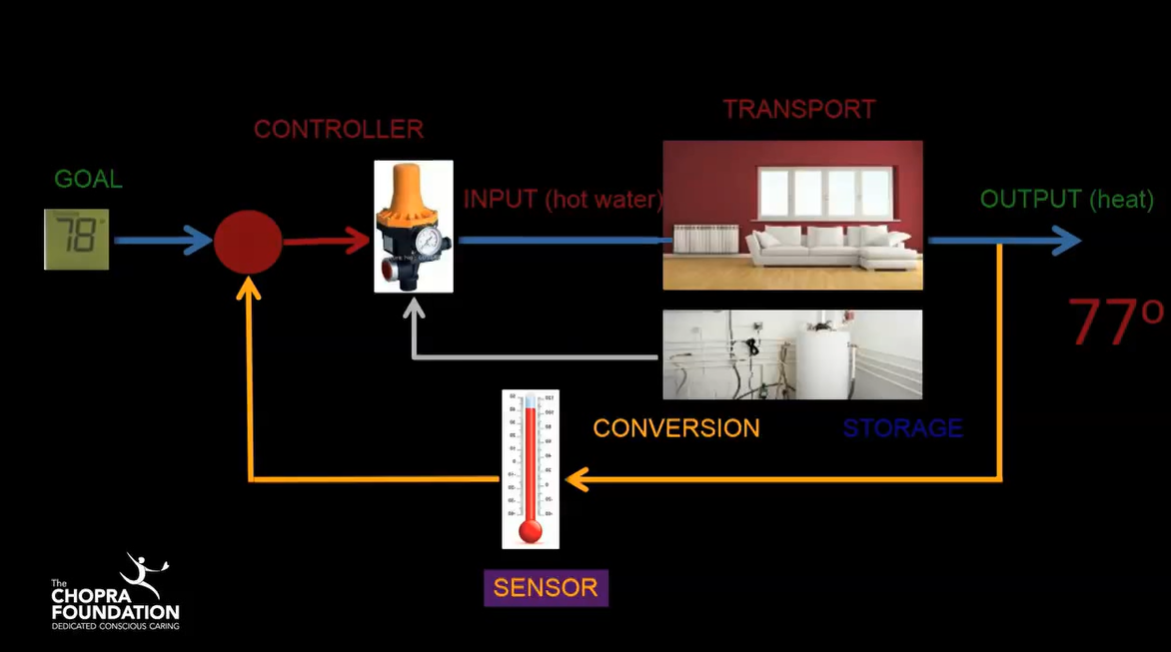
\includegraphics[width=\linewidth,keepaspectratio]{SystemsDiagram_Intelligent_Thermostat}

\end{center}	  
\end{frame}

%%%%%%%%%%%%%%%%%%%%%%%%%%%%%%%%%%%%%%%%%%%%%%%%%%%%%%%%%%%
\begin{frame}[fragile]\frametitle{Ayurveda through Systems Lens}
      \begin{itemize}
        \item Ayurveda’s concepts map to Control Systems Engineering:
          \begin{itemize}
            \item \textbf{Vata}: Transport function.
            \item \textbf{Pitta}: Conversion processes.
            \item \textbf{Kapha}: Structural and storage roles.
          \end{itemize}
        \item Feedback systems in Ayurveda personalize treatment.
        \item Karma as a dynamic system of cause and effect.
      \end{itemize}
\end{frame}


%%%%%%%%%%%%%%%%%%%%%%%%%%%%%%%%%%%%%%%%%%%%%%%%%%%%%%%%%%%
\begin{frame}[fragile]\frametitle{Ayurveda Systems Diagram}

\begin{center}
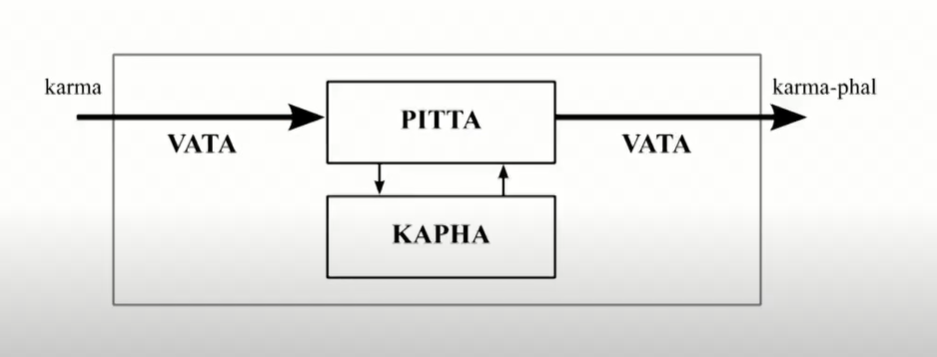
\includegraphics[width=0.8\linewidth,keepaspectratio]{SystemsDiagram_Ayurveda}

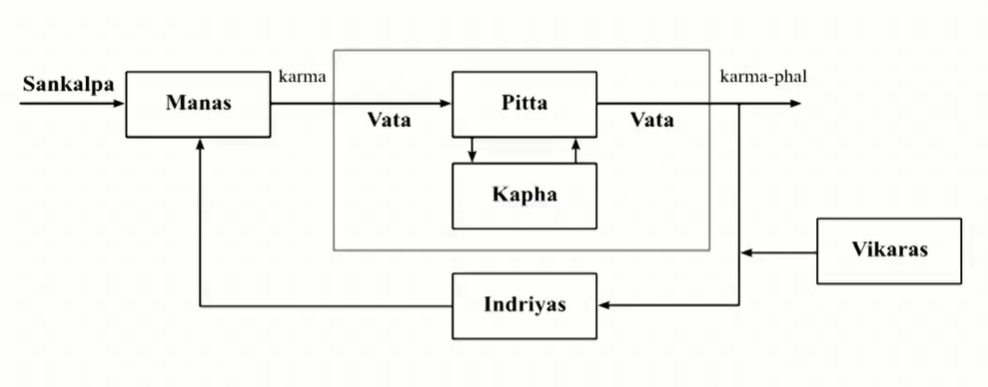
\includegraphics[width=0.8\linewidth,keepaspectratio]{SystemsDiagram_Intelligent_Ayurveda}

\end{center}	  
\end{frame}


%%%%%%%%%%%%%%%%%%%%%%%%%%%%%%%%%%%%%%%%%%%%%%%%%%%%%%%%%%%
\begin{frame}[fragile]\frametitle{Bridging Eastern and Western Sciences}
      \begin{itemize}
        \item Systems Biology in the West aims to create a holistic view of the body.
        \item Ayurveda and Siddha provide similar holistic frameworks.
        \item Control Systems Engineering serves as a Rosetta Stone to translate between the two.
        \item Modern validation reinforces the ancient system’s relevance today.
      \end{itemize}
\end{frame}
